\documentclass[12pt,addpoints,answers]{evalua}
\grado{1$^\circ$ de Secundaria}
\cicloescolar{2024-2025}
\materia{Matemáticas 1}
\unidad{1}
\title{Examen de la Unidad}
\aprendizajes{
        \item Convierte fracciones decimales a notación decimal y viceversa. Aproxima algunas fracciones no decimales usando la notación decimal. 
        \item Ordena fracciones y números decimales.
        \item Resuelve problemas de suma y resta con números enteros, fracciones y decimales positivos y negativos.
        \item Resuelve problemas de multiplicación con fracciones y decimales y de división con decimales.
}
\author{Prof.: Julio César Melchor Pinto}
\begin{document}
\begin{multicols}{2}
	\tableofcontents
\end{multicols}\newpage
\begin{questions}\large
	\addcontentsline{toc}{section}{Cálculos numéricos}
	\section*{Cálculos numéricos}

	\question[10] Realiza las siguientes operaciones de \textit{cálculo numérico}:

	\begin{parts}
		\begin{multicols}{2}
			\addcontentsline{toc}{subsection}{Suma de números}
			\subsection*{Suma de números}
			\part $\dfrac{3}{4}+\dfrac{3}{8}=$ \fillin[$\dfrac{9}{8}=1\dfrac{1}{8}$][0in]

			\addcontentsline{toc}{subsection}{Multiplicación de números}
			\subsection*{Multiplicación de números}
			\part $9.27\times 5.4=$ \fillin[$50.058$][0in]

			\addcontentsline{toc}{subsection}{Resta de números}
			\subsection*{Resta de números}
			\part $\dfrac{1}{2}-\dfrac{2}{5}=$ \fillin[$\dfrac{1}{10}$][0in]

			\addcontentsline{toc}{subsection}{División de números}
			\subsection*{División de números}
			\part $622.21\divisionsymbol 115=$ \fillin[$5.41$][0in]
		\end{multicols}

		\addcontentsline{toc}{subsection}{Resolución de problemas}
		\subsection*{Resolución de problemas}
		\part Si un dólar equivale a 19 pesos. ¿Cuántos dólares serán 1634 pesos? \fillin[$1634\divisionsymbol 19 =$ 86 dólares][0in]
	\end{parts}

	% \newpage
	\addcontentsline{toc}{section}{Fracciones}
	\section*{Fracciones}


	\addcontentsline{toc}{subsection}{Nombre de fracciones}
	\subsection*{Nombre de fracciones}

	\question[4] Escribe la fracción que corresponda en cada inciso:

	\begin{parts}
		% \part ¿Cómo se escribe numéricamente la fracción \textbf{ocho quintos}?    \fillin[$\dfrac{8}{5}$][0in]  \\
		\part ¿Cómo se escribe numéricamente la fracción \textbf{seis onceavos}?   \fillin[$\dfrac{6}{11}$][0in] \\
		% \part ¿Cómo se escribe numéricamente la fracción \textbf{dos séptimos}?    \fillin[$\dfrac{2}{7}$][0in]  \\
		\part ¿Cómo se escribe numéricamente la fracción \textbf{once medios}?     \fillin[$\dfrac{11}{2}$][0in] \\
		% \part ¿Cómo se escribe numéricamente la fracción \textbf{diez décimos}?    \fillin[$\dfrac{10}{10}$][0in]\\
	\end{parts}

	\addcontentsline{toc}{subsection}{Representación de fracciones}
	\subsection*{Representación de fracciones}

	\question[4]{Escribe sobre la línea la fracción que representa cada imagen:\\

		\begin{multicols}{4}
			\begin{parts}
				\part 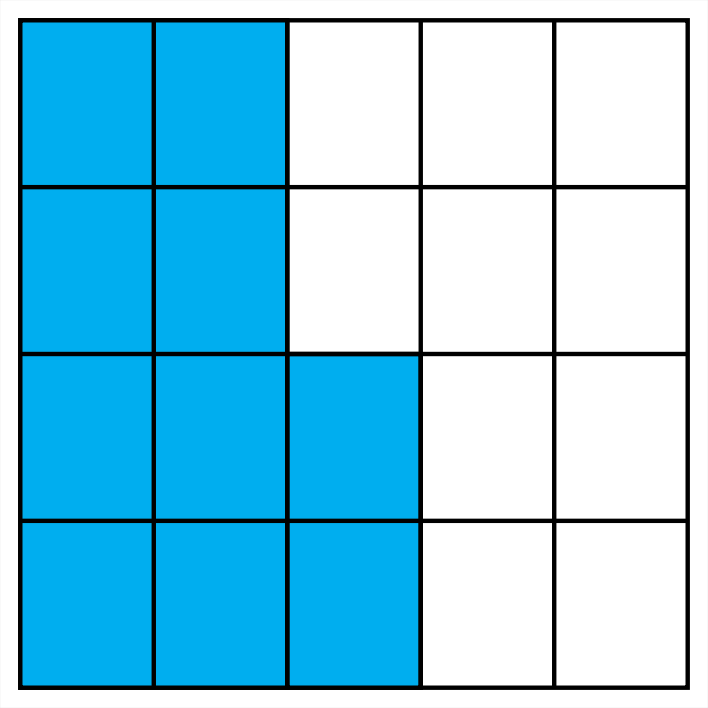
\includegraphics[width=48px]{../images/imagen_frac01.png} \fillin[\fbox{$\dfrac{10}{20}$}][0in]   \\[2em]
				\part 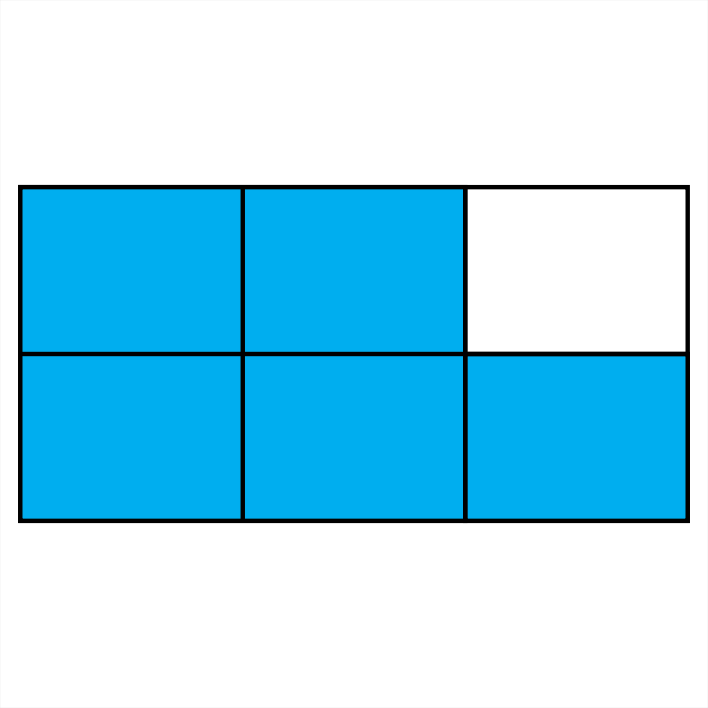
\includegraphics[width=48px]{../images/imagen_frac02.png} \fillin[\fbox{$\dfrac{5}{6}$}][0in]     \\[2em]
				% \part 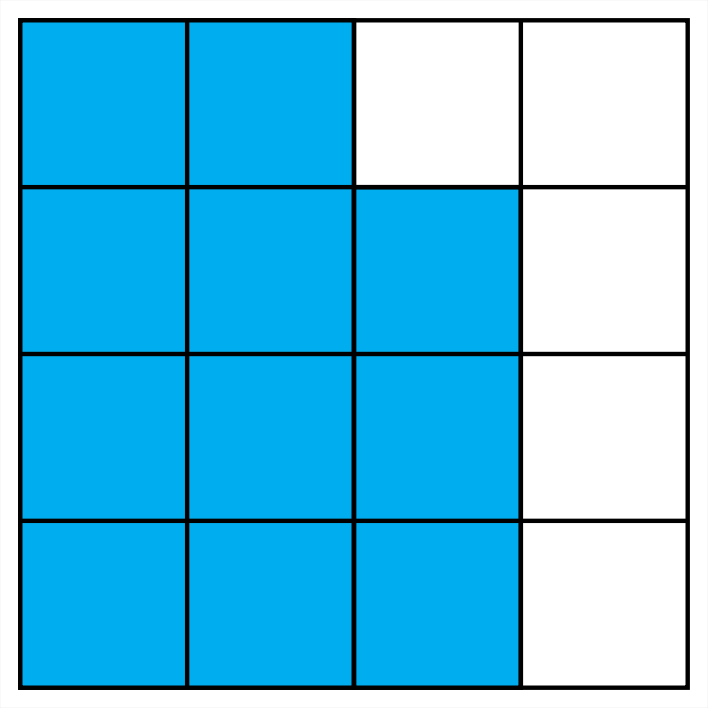
\includegraphics[width=48px]{../images/imagen_frac03.png} \fillin[\fbox{$\dfrac{11}{16}$}][0in]   \\[2em]
				% \part 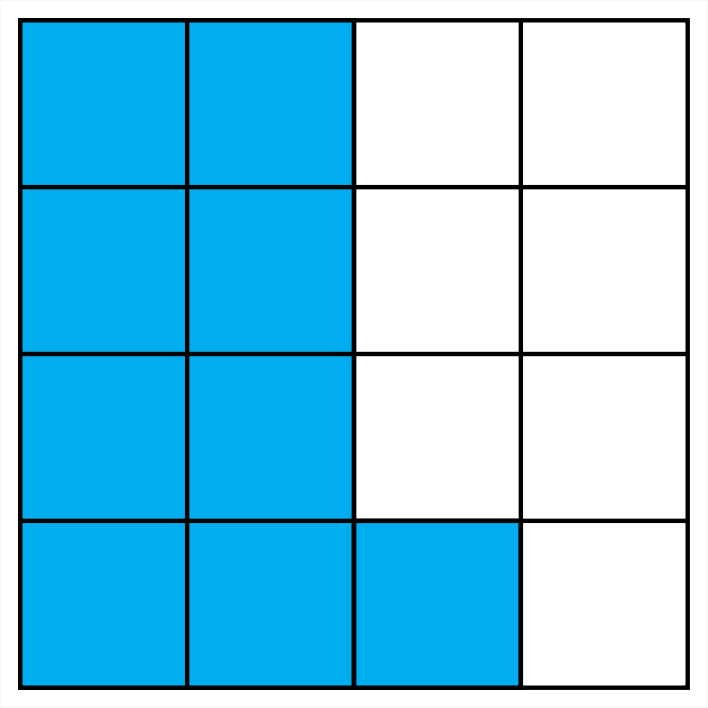
\includegraphics[width=48px]{../images/imagen_frac06.png} \fillin[\fbox{$\dfrac{9}{16}$}][0in]    \\[2em]
				% \part 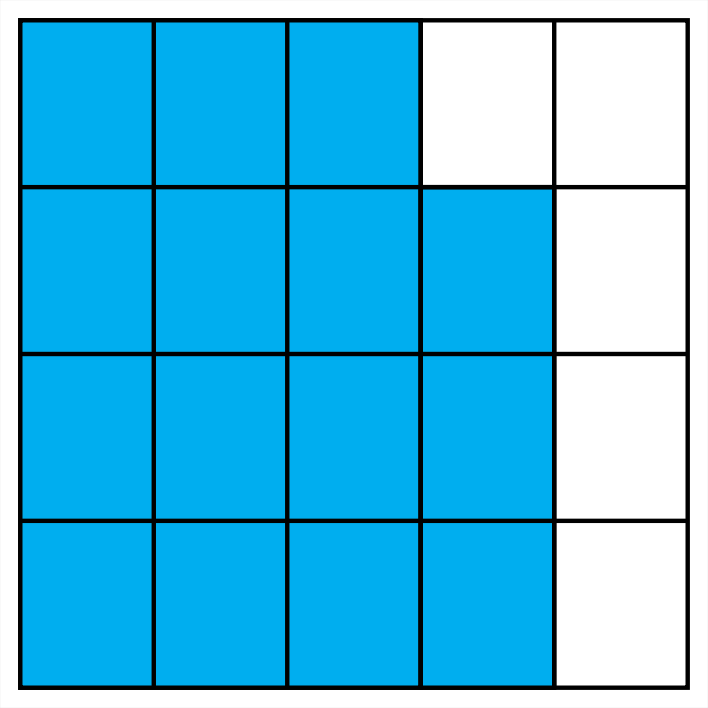
\includegraphics[width=48px]{../images/imagen_frac07.png} \fillin[\fbox{$\dfrac{15}{20}$}][0in]   \\[2em]
				% \part 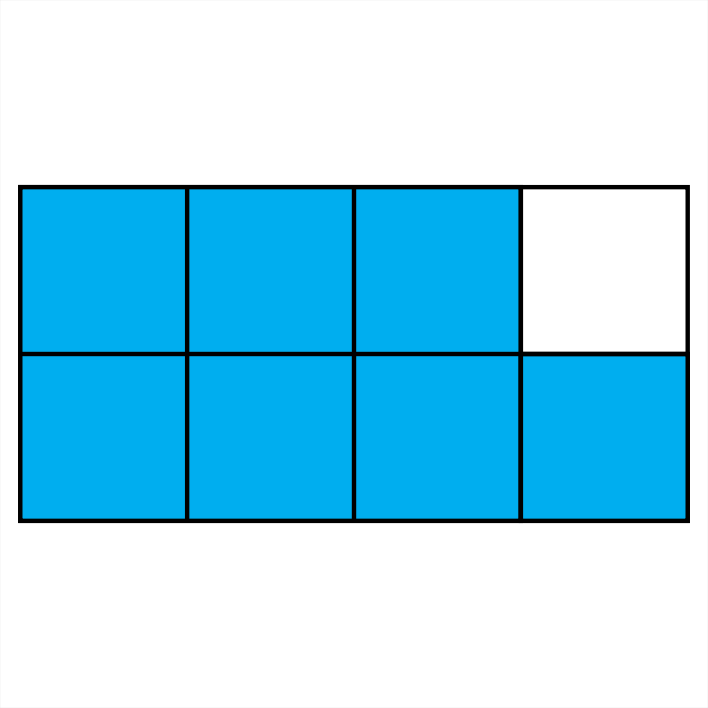
\includegraphics[width=48px]{../images/imagen_frac08.png} \fillin[\fbox{$\dfrac{7}{8}$}][0in]     \\[2em]
				\part 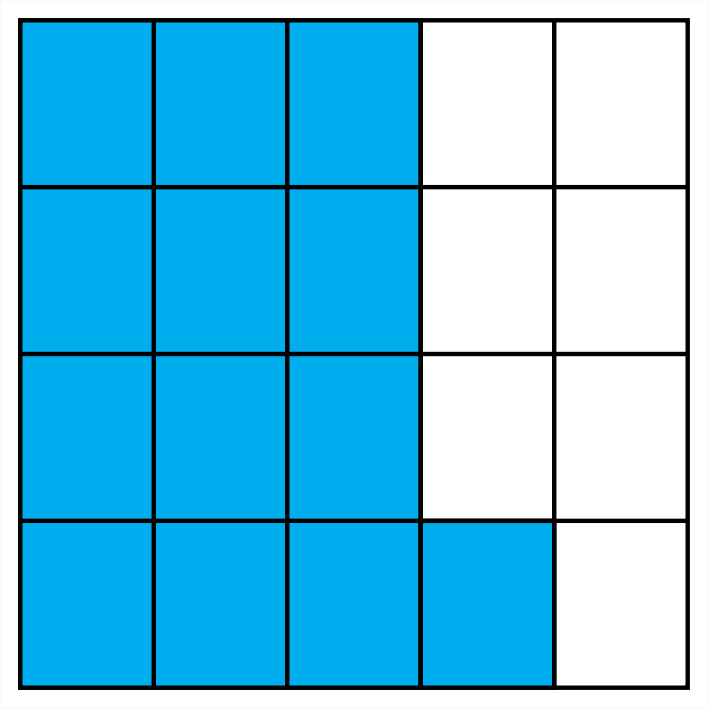
\includegraphics[width=48px]{../images/imagen_frac09.png} \fillin[\fbox{$\dfrac{13}{20}$}][0in]   \\[2em]
				\part 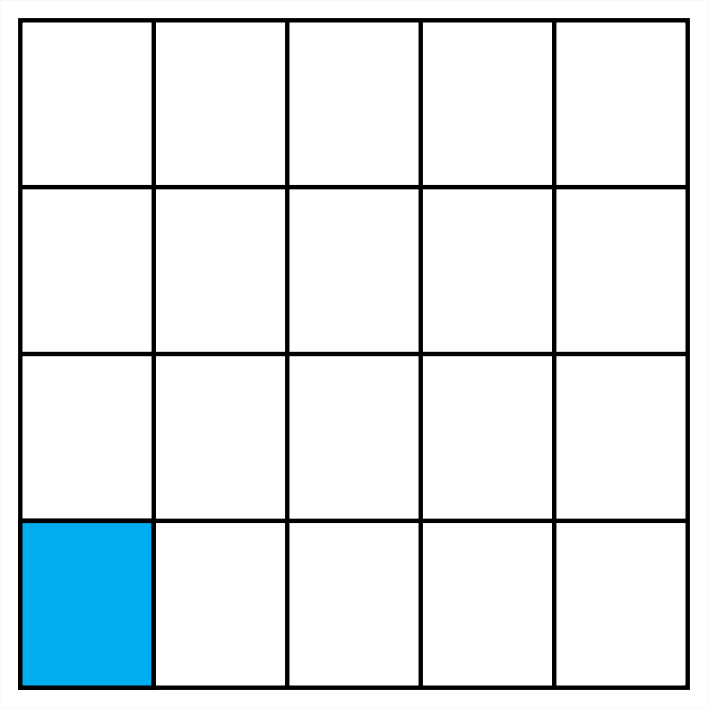
\includegraphics[width=48px]{../images/imagen_frac11.png} \fillin[\fbox{$\dfrac{1}{20}$}][0in]    \\[2em]
			\end{parts}
		\end{multicols}
	}

	\addcontentsline{toc}{subsection}{Clasificación de fracciones}
	\subsection*{Clasificación de fracciones}

	\question[4]{Clasifica las siguientes fracciones en propias, impropias o mixtas:

		\begin{multicols}{4}
			\begin{parts}%\large
				\part $\dfrac{5}{6}$   \fillin[Propia][1.5cm]   \\[2em]
				\part $5\dfrac{5}{11}$ \fillin[Mixta][1.5cm]   \\[1em]
				\part $1\dfrac{2}{3}$  \fillin[Mixta][1.5cm]    \\[2em]
				\part $\dfrac{3}{4}$   \fillin[Propia][1.5cm]  \\[1em]
				\part $\dfrac{7}{5}$   \fillin[Impropia][1.5cm] \\[2em]
				\part $\dfrac{7}{8}$   \fillin[Propia][1.5cm]   \\[1em]
				\part $\dfrac{3}{2}$   \fillin[Impropia][1.5cm] \\[2em]
				\part $4\dfrac{1}{4}=$ \fillin[Mixta][1.5cm]   \\[1em]
			\end{parts}
		\end{multicols}
	}



	\addcontentsline{toc}{subsection}{Fracciones en la recta numérica}
	\subsection*{Fracciones en la recta numérica}

	\question[4] Escribe la fracción que representa el punto en la recta numérica

	\begin{multicols}{2}
		\begin{parts}
			\part 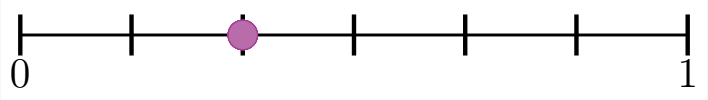
\includegraphics[width=150px]{../images/recta_num_frac01.png} \\[-0.5em] \fillin[$\dfrac{2}{6}$][2in]
			\part 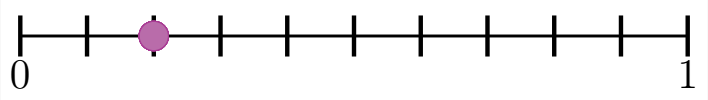
\includegraphics[width=150px]{../images/recta_num_frac02.png} \\[-0.5em] \fillin[$\dfrac{2}{10}$][2in]
			% \part 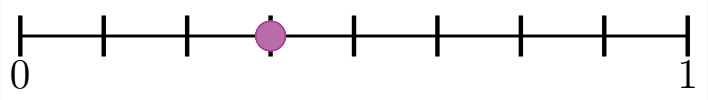
\includegraphics[width=150px]{../images/recta_num_frac03.png} \\[-0.5em] \fillin[$\dfrac{2}{6}$][1.5in]
			% \part 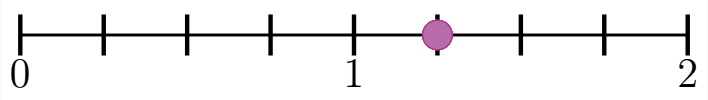
\includegraphics[width=150px]{../images/recta_num_frac04.png} \\[-0.5em] \fillin[$\dfrac{2}{6}$][1.5in]
			% \part 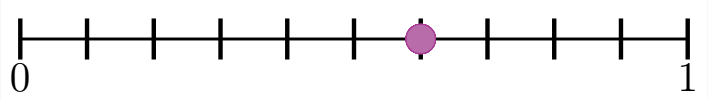
\includegraphics[width=150px]{../images/recta_num_frac05.png} \\[-0.5em] \fillin[$\dfrac{2}{6}$][1.5in]
			% \part 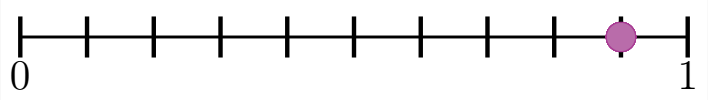
\includegraphics[width=150px]{../images/recta_num_frac06.png} \\[-0.5em] \fillin[$\dfrac{2}{6}$][1.5in]
			% \part 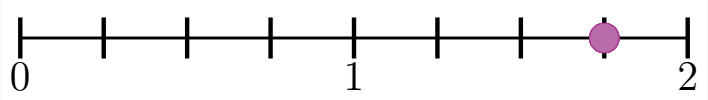
\includegraphics[width=150px]{../images/recta_num_frac07.png} \\[-0.5em] \fillin[$\dfrac{2}{6}$][1.5in]
			% \part 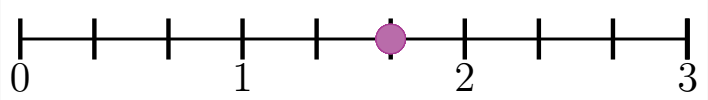
\includegraphics[width=150px]{../images/recta_num_frac08.png} \\[-0.5em] \fillin[$\dfrac{2}{6}$][1.5in]
			% \part 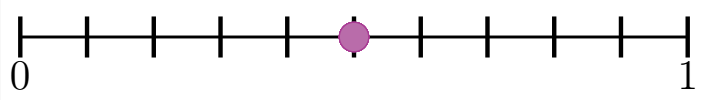
\includegraphics[width=150px]{../images/recta_num_frac09.png} \\[-0.5em] \fillin[$\dfrac{2}{6}$][1.5in]
			% \part 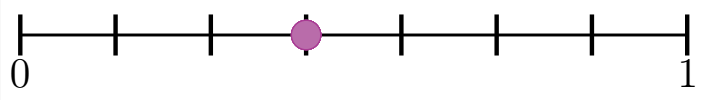
\includegraphics[width=150px]{../images/recta_num_frac10.png} \\[-0.5em] \fillin[$\dfrac{2}{6}$][1.5in]
		\end{parts}
	\end{multicols}

	\addcontentsline{toc}{subsection}{Conversión de fracciones}
	\subsection*{Conversión de fracciones}

	\question[4] Convierte la siguientes fracciones impropias a mixtas:

	\begin{multicols}{3}
		\begin{parts}
			\part $\dfrac{13}{3}= $ \fillin[$4\dfrac{1}{3}$][0in]
			% \part $\dfrac{63}{10}= $ \fillin[$6\dfrac{3}{10}$][0in]
			\part $\dfrac{51}{5}= $ \fillin[$10\dfrac{1}{5}$][0in]
		\end{parts}
	\end{multicols}

	% \newpage
	\addcontentsline{toc}{section}{Fracciones, M.C.M. y M.C.D.}
	\section*{Fracciones, M.C.M. y M.C.D.}

	\addcontentsline{toc}{subsection}{Comparación de fracciones}
	\subsection*{Comparación de fracciones}

	\question[8] Compara las siguientes fracciones usando los signos mayor que (>), menor que (<) o igual (=):

	\begin{multicols}{4}
		\begin{parts}
			\part $\dfrac{4}{3}$ \fillin[$>$][0.5in] $\dfrac{5}{4}$\\[0.75em]
			\part $\dfrac{1}{3}$ \fillin[$=$][0.5in] $\dfrac{3}{9}$\\[0.75em]
			% \part $\dfrac{2}{3}$ \fillin[$<$][0.5in] $\dfrac{3}{2}$\\[0.75em]
			% \part $\dfrac{3}{4}$ \fillin[$>$][0.5in] $\dfrac{2}{3}$\\[0.75em]
			\part $\dfrac{5}{6}$ \fillin[$>$][0.5in] $\dfrac{4}{5}$\\[0.75em]
			\part $\dfrac{1}{3}$ \fillin[$<$][0.5in] $\dfrac{2}{5}$\\[0.75em]
		\end{parts}
	\end{multicols}

	\addcontentsline{toc}{subsection}{Fracciones equivalentes}
	\subsection*{Fracciones equivalentes}

	\question[8] Indica si las siguientes fracciones son equivalentes o no:

	\begin{multicols}{2}
		\begin{parts}
			\part $\dfrac{4}{5}=\dfrac{8}{10}$\qquad
			\begin{oneparcheckboxes}
				\CorrectChoice Sí
				\choice No
			\end{oneparcheckboxes}

			\part $\dfrac{1}{8}=\dfrac{4}{16}$\qquad
			\begin{oneparcheckboxes}
				\choice Sí
				\CorrectChoice No
			\end{oneparcheckboxes}

			\part $\dfrac{1}{5}=\dfrac{5}{10}$\qquad
			\begin{oneparcheckboxes}
				\choice Sí
				\CorrectChoice No
			\end{oneparcheckboxes}

			\part $\dfrac{1}{10}=\dfrac{3}{30}$\qquad
			\begin{oneparcheckboxes}
				\CorrectChoice Sí
				\choice No
			\end{oneparcheckboxes}
		\end{parts}
	\end{multicols}

	\addcontentsline{toc}{subsection}{M.C.D y M.C.M}
	\subsection*{M.C.D y M.C.M}
	\question[4] Calcula lo que se te pide en cada inciso:

	\begin{multicols}{2}
		\begin{parts}
			\part Encuentra el máximo común divisor de 120 y 300.

			\begin{solutionbox}{1.4cm}
				Se calcula el MCD$(120,300) = 60$.
			\end{solutionbox}

			\part Encuentra el mínimo común múltiplo de 12, 15 y 18.

			\begin{solutionbox}{1.4cm}
				Se calcula el MCM$(12,15,18) = 180$.
			\end{solutionbox}

		\end{parts}
	\end{multicols}

	\newpage
	\addcontentsline{toc}{subsection}{Simplificación de fracciones}
	\subsection*{Simplificación de fracciones}

	\question[4] Simplifica a su mínima expresión la siguiente fracción usando el máximo común divisor

	\begin{multicols}{2}
		\begin{parts}
			\part $\dfrac{8}{64}=$ \fillin[$\dfrac{1}{8}$][0in]
			\part $\dfrac{6}{42}=$ \fillin[$\dfrac{1}{7}$][0in]
		\end{parts}
	\end{multicols}

	\addcontentsline{toc}{subsection}{Resolución de problemas}
	\subsection*{Resolución de problemas}

	\question[6] María y Jorge tienen 45 bolas blancas, 15 bolas azules y 90 bolas rojas y quieren hacer el mayor número de collares iguales sin que sobre ninguna bola. ¿Cuántos collares iguales pueden hacer?

	\begin{solutionbox}{2cm}
		Se calcula el M.C.D.$(45,15,90) = 15$.\\
		Por lo tanto, se pueden hacer 15 collares.
	\end{solutionbox}

	\addcontentsline{toc}{section}{Números decimales}
	\section*{Números decimales}

	\addcontentsline{toc}{subsection}{Ubicación en la recta numérica}
	\subsection*{Ubicación en la recta numérica}

	\question[4] Escribe el número que representa el punto indicado en la recta numérica de cada uno de los siguientes incisos.

	\begin{multicols}{2}
		\begin{parts}
			\part 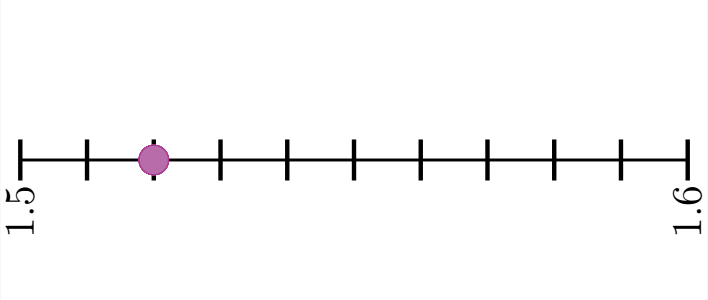
\includegraphics[width=140px]{../images/recta_num_1.52.png} \\[-0.5em] \fillin[$1.52$][1.5in]
			\part 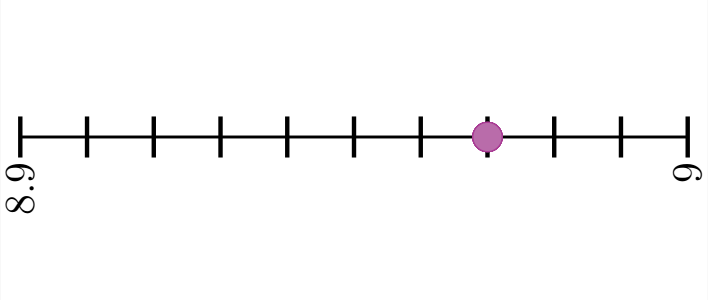
\includegraphics[width=140px]{../images/recta_num_8.97.png} \\[-0.5em]  \fillin[$8.97$][1.5in]  \\[-1.4em]
		\end{parts}
	\end{multicols}

	\addcontentsline{toc}{subsection}{Porcentajes a decimal}
	\subsection*{Porcentajes a decimal}

	\question[4] Escribe el número decimal que representa cada porcentaje:

	% \begin{multicols}{2}
	\begin{parts}	\normalsize
		\part Convierte 22.9\% a un número decimal. \fillin[$0.229$][0in]
		\part Convierte 6.2\% a un número decimal. \fillin[$0.062$][0in]
	\end{parts}
	% \end{multicols}

	\addcontentsline{toc}{subsection}{Operaciones con múltiplos de 10}
	\subsection*{Operaciones con múltiplos de 10}

	\question[4] Realiza las siguientes operaciones con múltiplos de 10:

	\begin{multicols}{2}
		\begin{parts}\normalsize
			\part $56.9 \times 100=$ \fillin[$5690$][0in]
			\part $0.712 \times 1000=$ \fillin[$712$][0in]
		\end{parts}
	\end{multicols}

	\newpage
	\addcontentsline{toc}{subsection}{Conversión de fracciones a decimales}
	\subsection*{Conversión de fracciones a decimales}

	\question[4] Convierte las siguientes fracciones a decimales:

	\begin{multicols}{2}
		\begin{parts}\normalsize
			\part $\dfrac{7}{20}=$ \fillin[$0.35$][0in]
			\part $\dfrac{1927}{1000}=$ \fillin[$1.927$][0in]
		\end{parts}
	\end{multicols}

	\addcontentsline{toc}{subsection}{Conversión de decimales a fracciones}
	\subsection*{Conversión de decimales a fracciones}

	\question[4] Convierte los siguientes números decimales a una fracción simplificada a su mínima expresión:

	\begin{multicols}{2}
		\begin{parts}\normalsize
			\part $0.04=$ \fillin[$\dfrac{1}{25}$][0in]
			\part $0.19=$ \fillin[$\dfrac{19}{100}$][0in]
		\end{parts}
	\end{multicols}

	% \newpage

	\addcontentsline{toc}{section}{Números negativos}
	\section*{Números negativos}
	\addcontentsline{toc}{subsection}{Ubicación en la recta numérica}
	\subsection*{Ubicación en la recta numérica}

	\question[4] Escribe el número que representa el punto indicado en la recta numérica de cada uno de los siguientes incisos.

	\begin{multicols}{2}
		\begin{parts}
			\part 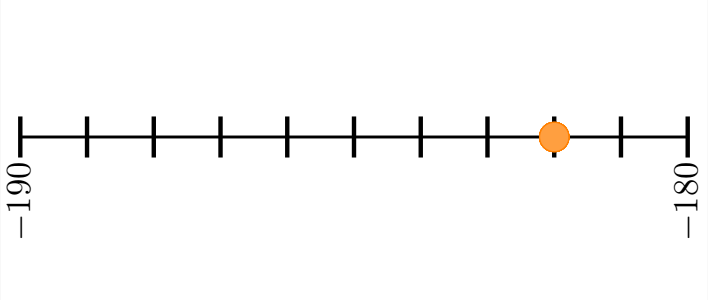
\includegraphics[width=140px]{../images/recta_num_-182.png} \\[-1em]   \fillin[$-182$][1.5in]
			\part 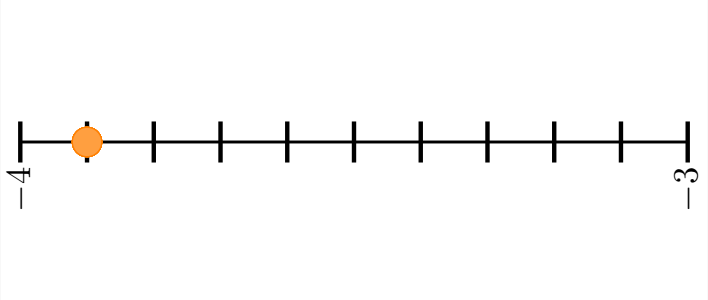
\includegraphics[width=140px]{../images/recta_num_-3.9.png} \\[-1em]  \fillin[$-3.9$][1.5in]
		\end{parts}
	\end{multicols}

	\addcontentsline{toc}{subsection}{Comparación de negativos}
	\subsection*{Comparación de negativos}

	\question[4] Escribe sobre la línea el símbolo de mayor que ($>$), menor que ($<$), o igual ($=$) según corresponda.

	\begin{multicols}{2}
		\begin{parts}\normalsize
			\part $-182$ \fillin[$>$][0.5in] $-189$
			\part $-97$ \fillin[$<$][0.5in] $-96.2$
		\end{parts}
	\end{multicols}

	\addcontentsline{toc}{subsection}{Determina el signo}
	\subsection*{Determina el signo}

	\question[4] Determina el signo \textit{positivo} o \textit{negativo} que resulta de las siguientes operaciones:

	\begin{multicols}{2}
		\begin{parts}\normalsize
			\part $-28-19$ \fillin[Negativo][1in]
			\part $-43+55$ \fillin[Positivo][1in]
		\end{parts}
	\end{multicols}

	\addcontentsline{toc}{subsection}{Suma y resta con negativos}
	\subsection*{Suma y resta con negativos}

	\question[4] Realiza las siguientes operaciones con números negativos:

	\begin{multicols}{2}
		\begin{parts}\normalsize
			\part $-223+67=$ \fillin[$-156$][0in]
			\part $(16)-(-14)$ \fillin[$30$][0in]
		\end{parts}
	\end{multicols}
\end{questions}
\end{document}
